\chapter{Symmetry, Supersymmetry, and Grassmann Numbers}

We begin, as Leonard Susskind does in this lecture, by backing up before going forward. Before supersymmetry can be introduced as a strange new symmetry, we must remind ourselves what an ordinary symmetry is, how it acts on quantum states, how its infinitesimal generators close into a commutator algebra, and why a genuine symmetry must leave the energy unchanged. Only then does the lecture make its decisive turn: ordinary symmetries preserve bosons as bosons and fermions as fermions, while supersymmetry mixes the two. These companion notes follow Leonard Susskind's Lecture 4 closely and are curated by LazyingArt LLC.

\section{Symmetries As Operations On States}

A symmetry relates configurations that differ by a transformation. In that plain sense, symmetry is already a statement about sameness hidden inside difference. Left and right hands, if the world were exactly left-right symmetric, would be related in precisely this way: different configurations, but tied together by a transformation, and therefore carrying the same physical properties. One of the lecture's first reminders is that such symmetry relations generally enforce equal masses or equal energies for the states they connect.

In quantum mechanics the language sharpens immediately. A physical system is represented by a state vector, and a symmetry is represented by an operator acting on that state vector. We do not begin by rotating the Hilbert space for its own sake; rather, we represent a physical rotation, translation, or other transformation by an operator acting on states. If the transformation is denoted by \(U\), then the transformed state is schematically of the form
\begin{equation}
U|\psi\rangle.
\end{equation}
The board at this point is partially occluded in the surviving frame, but the intended passage is clear: transformed-state notation first, then the algebraic condition that makes \(U\) a legitimate symmetry operator.

\begin{figure}[t]
\centering

\includegraphics[width=0.58\textwidth]{lecture_04_figure_02.png}
\caption{Early unitary-operator notation on the board.}
\end{figure}

The essential condition is unitarity:
\begin{equation}
U^\dagger U = 1.
\end{equation}
This is not an ornamental mathematical adjective. It is the statement that the Hermitian conjugate is the inverse,
\begin{equation}
U^\dagger = U^{-1},
\end{equation}
and therefore that state vectors preserve their norm under the transformation. In the lecture this is stated in the most physical way possible: unitarity is just the conservation of probability.

\subsection{Question \& Answer: Are We Rotating Space or Hilbert Space?}

A natural question arises immediately. If a state vector is an element of Hilbert space, then when we speak about a rotation are we rotating three-dimensional space or are we rotating the Hilbert space?

The lecture's answer is: both, but not in the same sense. The physical operation is a rotation in space. The mathematical representation of that operation is a unitary transformation acting in Hilbert space. The Hilbert-space transformation is the representation of the spatial rotation. It is therefore better to say that \(U\) acts on states, while representing the act of rotating the physical configuration.

\section{Infinitesimal Transformations And Generators}

Once \(U\) has been introduced as a symmetry operator, the lecture narrows its focus to very small transformations. This is where continuous symmetry becomes tractable. No transformation at all is represented by
\begin{equation}
U=1,
\end{equation}
not by \(U=0\). So if we rotate by a very small angle \(\epsilon\), or translate by a very small amount \(\epsilon\), the operator must differ from the identity only slightly:
\begin{equation}
U(\epsilon)=1+i\epsilon L+O(\epsilon^2).
\end{equation}
The operator \(L\) must be Hermitian,
\begin{equation}
L^\dagger=L,
\end{equation}
because that is precisely what is needed to make \(U(\epsilon)\) unitary to leading order in \(\epsilon\).

For rotations, the generators must carry directional labels. We may speak of \(L_x\), \(L_y\), and \(L_z\), corresponding to infinitesimal rotations about the three coordinate axes. An arbitrary infinitesimal rotation is then built from a linear combination of these basic generators. In the lecture Susskind insists on this point: rotations about arbitrary axes are not new objects; they are assembled from the three elementary generators.

For spatial rotations these generators are, of course, angular momentum operators. But the notation \(L_i\) is useful here because the lecture is still emphasizing the general theory of symmetry before specializing to supersymmetry.

\section{Why Commutators Encode The Group}

The next step is the real algebraic heart of the recap. A continuous group is not summarized by a list of finite transformations. It is summarized by the infinitesimal generators and, more specifically, by their commutator algebra. For rotations the abstract statement is
\begin{equation}
[L_i,L_j]=i\epsilon_{ijk}L_k.
\end{equation}
But Susskind does not want to leave this as a bare formula. He wants to show what a commutator means geometrically.

\paragraph{A worked small-rotation loop.}

Take a small rotation about the \(x\)-axis and then a small rotation about the \(y\)-axis:
\begin{equation}
U_x(\epsilon)=1+i\epsilon L_x,
\qquad
U_y(\delta)=1+i\delta L_y.
\end{equation}
Now perform the loop
\begin{equation}
U_x(\epsilon)\,U_y(\delta)\,U_x^{-1}(\epsilon)\,U_y^{-1}(\delta).
\end{equation}
If rotations about different axes commuted, this would collapse to the identity. The lecture dwells on the fact that it does not. The full spoken expansion contains false starts and a brief factor-of-two confusion, but the cleaned endpoint is the important part:
\begin{equation}
U_x(\epsilon)\,U_y(\delta)\,U_x^{-1}(\epsilon)\,U_y^{-1}(\delta)
=
1+i\epsilon\delta L_z+O(\epsilon^2,\delta^2).
\end{equation}
So the failure of cancellation is itself another infinitesimal rotation, here about the \(z\)-axis. That is the content of the commutator. The commutator measures the non-cancellation of doing one small operation, then another, and then undoing them in reverse.

From here the lecture broadens the discussion from rotations to translations. A small translation along the \(x\)-axis is generated by momentum:
\begin{equation}
T_x(\epsilon)=1+i\epsilon P_x,
\qquad
T_y(\epsilon)=1+i\epsilon P_y.
\end{equation}
Now the geometry changes. Translate in \(x\), then in \(y\), then undo \(x\), then undo \(y\), and one returns to the same point. In Euclidean space translations commute, so
\begin{equation}
[P_i,P_j]=0.
\end{equation}

Rotations and translations, however, do not commute. If we translate a point and then rotate it, undo the translation, and then undo the rotation, we do not come back to the same place. The lecture gives the standard infinitesimal conclusion only schematically; in normalized form it is
\begin{equation}
[L_i,P_j]=i\epsilon_{ijk}P_k.
\end{equation}
The precise spoken notation is rough, but the point is stable: once the commutators are known, the local structure of the whole group is known. The commutator algebra is the multiplication table of the group written in infinitesimal form.

\section{Symmetry And The Hamiltonian}

Having reviewed how symmetry transformations combine, the lecture makes its central dynamical pivot. A genuine symmetry should not change the energy of a state. This is first said naively and physically: if one simply rotates a system, or simply translates the whole system, the energy should not change. Then the lecture turns that intuition into a precise operator condition.

We begin with an energy eigenstate. The board isolates the transformed state and the eigenvalue equation in two very sparse but very useful moments.

\begin{figure}[t]
\centering

\includegraphics[width=0.48\textwidth]{lecture_04_figure_03.png}
\caption{Symmetry operator acting on an energy eigenstate.}
\end{figure}

\begin{figure}[t]
\centering

\includegraphics[width=0.52\textwidth]{lecture_04_figure_04.png}
\caption{Hamiltonian eigenvalue equation.}
\end{figure}

The defining relation is
\begin{equation}
H|E\rangle = E|E\rangle.
\end{equation}
Here the lecture uses the same symbol \(E\) both for the scalar eigenvalue and for the label in the ket \(|E\rangle\). We will keep that notation locally, because it is the lecture's notation, but the distinction must be kept verbally clear: the \(E\) multiplying the ket is a number, while \(|E\rangle\) is the state.

If \(U\) is a symmetry, then the transformed state \(U|E\rangle\) must have the same energy. Therefore
\begin{align}
H|E\rangle &= E|E\rangle, \\
HU|E\rangle &= E\,U|E\rangle.
\end{align}
Now the lecture pauses, restarts, and goes through the logic a second time, because the key move is easy to lose sight of. Since the scalar \(E\) commutes with the operator \(U\), we may rewrite
\begin{equation}
E\,U|E\rangle = U\,E|E\rangle = UH|E\rangle.
\end{equation}
Hence
\begin{equation}
(HU-UH)|E\rangle = 0.
\end{equation}

\begin{figure}[t]
\centering

\includegraphics[width=0.70\textwidth]{lecture_04_figure_05.png}
\caption{From the transformed eigenstate to a commutator condition.}
\end{figure}

To preserve the visual rhythm of the board, it is worth displaying the same derivation in a clean companion layout:

\begin{figure}[t]
\centering
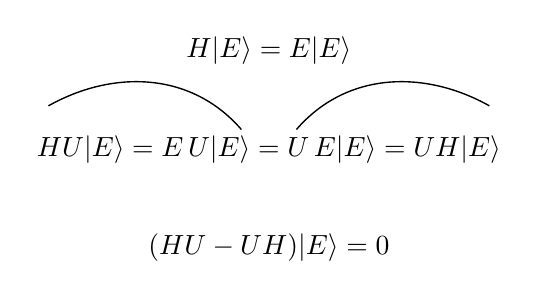
\begin{tikzpicture}
\node at (0,2.6) {$H|E\rangle = E|E\rangle$};
\node at (0,1.35) {$HU|E\rangle = E\,U|E\rangle = U\,E|E\rangle = UH|E\rangle$};
\node at (0,0.1) {$(HU-UH)|E\rangle = 0$};
\draw[line width=0.5pt] (-2.8,1.9) .. controls (-2.0,2.35) and (-1.0,2.35) .. (-0.35,1.6);
\draw[line width=0.5pt] (2.8,1.9) .. controls (2.0,2.35) and (1.0,2.35) .. (0.35,1.6);
\end{tikzpicture}
\caption{A clean companion reconstruction of the board derivation; the curved lines only echo the lecture's guide marks.}
\end{figure}

If this holds for every energy eigenstate, and if the energy eigenstates form a complete basis, then the operator itself must vanish:
\begin{equation}
[U,H]=0.
\end{equation}
That is the criterion for a symmetry in quantum mechanics. A legitimate symmetry operator commutes with the Hamiltonian.

The last step is immediate. If
\begin{equation}
U(\epsilon)=1+i\epsilon L_i+O(\epsilon^2),
\end{equation}
and every such \(U\) commutes with \(H\), then the generators must commute with \(H\) as well:
\begin{equation}
[L_i,H]=0.
\end{equation}
The lower label on the surviving board image is not perfectly sharp, but the normalized form \([L_i,H]=0\) is the safest statement.

\begin{figure}[t]
\centering

\includegraphics[width=0.45\textwidth]{lecture_04_figure_06.png}
\caption{Symmetry operators and generators commuting with the Hamiltonian.}
\end{figure}

Commutation with the Hamiltonian is not merely a kinematic curiosity. In the Heisenberg sense it is the statement of conservation:
\begin{equation}
[O,H]=0
\qquad \Longrightarrow \qquad
\dot O = 0.
\end{equation}
Thus symmetry and conservation law are two sides of the same structure.

The lecture immediately applies this to atomic degeneracy. At fixed total angular momentum \(l\), the different magnetic quantum numbers \(m\) are rotated into one another, and therefore have the same energy:
\begin{equation}
E_{l,m}=E_l.
\end{equation}
This is precisely what rotational symmetry buys us, so long as no external field breaks the symmetry.

\subsection{Question \& Answer: What Counts As A True Symmetry?}

A dangerous misunderstanding appears here, and the lecture spends real time clearing it away.

Take a spin with no external field. Rotate it, and nothing happens to its energy. Good. Now put the spin in a magnetic field and rotate only the spin. Its energy changes. Does that mean rotations are not symmetries? No. It means we did not perform the symmetry operation. We rotated one part of the setup relative to something we left fixed. A true symmetry operation would rotate the spin and the magnetic field together.

The same correction appears again for translation. An electron in the field of a proton does not keep the same energy if we translate only the electron. But that is not the symmetry operation. Translating the entire configuration is the symmetry. In other words, when the lecture says that a symmetry does not change the energy, it means a transformation of the whole system, including whatever fields or background structures belong to the physical setup.

\section{Why Supersymmetry Is Different}

Only after this entire recap does the lecture introduce the new ingredient. All of the symmetries discussed so far have one common feature: they preserve particle type. A rotation takes an electron to an electron, not to a photon. A color transformation takes a quark to a quark, not to a gluon. More generally, the familiar symmetries preserve the bosonic or fermionic character of a state, and they do not change the spin by half a unit.

Supersymmetry breaks that pattern. It is a symmetry whose generators take bosons into fermions and fermions into bosons. This is why the lecture treats it as something genuinely wild rather than as just one more internal symmetry. The mathematics is non-classical from the start, and ordinary geometric intuition is of little help.

The physical motivation is also stated very directly. If a theory enjoys supersymmetry, then bosonic and fermionic partners come in with equal mass. That is precisely the sort of pairing one would want if bosonic and fermionic contributions are to cancel the large renormalization effects discussed earlier in the course. In that sense the lecture does not introduce supersymmetry as a decorative mathematical extension; it is introduced as a candidate solution to a real dynamical problem.

\section{Supersymmetry Generators And Statistics}

To make the idea concrete, the lecture builds a prototype generator from creation and annihilation operators. Let \(A\) and \(A^\dagger\) be bosonic annihilation and creation operators, and \(C\) and \(C^\dagger\) the corresponding fermionic ones. Then the simplest operator with the right qualitative action is
\begin{equation}
Q = C^\dagger A + A^\dagger C.
\end{equation}
The first term annihilates a boson and creates a fermion. The second annihilates a fermion and creates a boson. In that schematic sense,
\begin{equation}
Q|B\rangle \sim |F\rangle,
\qquad
Q|F\rangle \sim |B\rangle.
\end{equation}
The lecture is careful here: \(Q\) is an operator, not a state. If it acts on a general superposition, it produces another superposition, but that is just ordinary linearity. The novelty is not that \(Q\) is some mixed boson-fermion state; the novelty is that it intertwines bosonic and fermionic sectors.

\subsection{Question \& Answer: What Happens When \(Q\) Acts On The Vacuum?}

The lecture pauses over the vacuum because this is exactly the kind of place where one can reason too quickly.

Apply
\begin{equation}
Q = C^\dagger A + A^\dagger C
\end{equation}
to the vacuum \(|0\rangle\). The operator \(A\) tries to annihilate a boson, but there is no boson in the vacuum. The operator \(C\) tries to annihilate a fermion, but there is no fermion there either. So
\begin{equation}
Q|0\rangle = 0.
\end{equation}
This is not the vacuum state again. It is the zero vector. The lecture emphasizes that distinction.

The next question is about spin. If a scalar boson is turned into a fermion, which fermion does one get? A spin-\(\tfrac12\) fermion has two components, so a single unindexed \(Q\) cannot be enough. This is why the supersymmetry generators must carry a spinor index:
\begin{equation}
Q_\alpha.
\end{equation}
The index itself is a half-spin index, because the generator changes the spin by half a unit. In the lecture this is stated in the most operational way: if \(Q\) acts on a spin-zero boson, there must be one component that produces the spin-up fermion and another that produces the spin-down fermion.

This leads to an important structural point. Supersymmetry generators are fermionic operators. They contain an odd number of fermion operators, and that is exactly what allows them to change bosons into fermions and fermions into bosons.

To see why this is a radical departure from ordinary observables, the lecture briefly reviews bosonic and fermionic operator algebra. For bosons we normalize the algebra as
\begin{align}
[A_i,A_j] &= 0, &
[A_i^\dagger,A_j^\dagger] &= 0, &
[A_i,A_j^\dagger] &= \delta_{ij}.
\end{align}
Thus bosonic creation operators commute:
\begin{equation}
A_i^\dagger A_j^\dagger = A_j^\dagger A_i^\dagger.
\end{equation}
A two-boson state is therefore symmetric under exchange of the labels \(i\) and \(j\).

For fermions the commutator is replaced by the anticommutator:
\begin{align}
\{C_i,C_j\} &= 0, &
\{C_i^\dagger,C_j^\dagger\} &= 0, &
\{C_i,C_j^\dagger\} &= \delta_{ij}.
\end{align}
In particular,
\begin{equation}
(C^\dagger)^2=0,
\end{equation}
which is the Pauli exclusion principle in operator form. And for two distinct labels,
\begin{equation}
C_i^\dagger C_j^\dagger = -\,C_j^\dagger C_i^\dagger.
\end{equation}
So fermionic two-particle states are antisymmetric under exchange.

This difference between bosonic and fermionic statistics is what forces the lecture toward a new arithmetic. Bosonic field amplitudes behave, in the classical limit, like ordinary commuting numbers. Fermionic objects do not. Their algebra suggests a different sort of number system altogether.

\section{Grassmann Numbers}

The lecture introduces Grassmann numbers as a bookkeeping device for fermionic quantities and for supersymmetry generators themselves. Ordinary numbers commute:
\begin{equation}
\alpha_i\alpha_j=\alpha_j\alpha_i.
\end{equation}
Grassmann numbers anticommute:
\begin{equation}
\theta_i\theta_j=-\,\theta_j\theta_i.
\end{equation}
In particular, setting \(i=j\) gives
\begin{equation}
\theta_i^2=0.
\end{equation}
Ordinary numbers commute with Grassmann numbers:
\begin{equation}
\alpha\theta=\theta\alpha.
\end{equation}

The lecture also distinguishes carefully between what is odd and what is even. A single \(\theta\) is Grassmann-odd. A product such as \(\theta_1\theta_2\) is Grassmann-even, in the sense that it commutes with other even quantities, but it is better not to call it an ordinary scalar in the naive sense, because it may still be nilpotent.

With only one Grassmann variable \(\theta\), the most general function is extremely simple:
\begin{equation}
f(\theta)=\alpha+\beta\theta.
\end{equation}
There is no quadratic term because \(\theta^2=0\). With two variables the most general polynomial function is
\begin{equation}
f(\theta_1,\theta_2)=\alpha+\beta_1\theta_1+\beta_2\theta_2+\gamma\theta_1\theta_2.
\end{equation}
That is already the whole space of functions. The lecture delights in how small this algebra is.

Differentiation is then defined so as to preserve the familiar product rule, at the price of one new sign convention. For one variable,
\begin{equation}
\partial_\theta(\alpha+\beta\theta)=\beta.
\end{equation}
For two variables,
\begin{equation}
\partial_{\theta_1}f=\beta_1+\gamma\theta_2,
\qquad
\partial_{\theta_2}f=\beta_2-\gamma\theta_1.
\end{equation}
The minus sign in the second formula is the whole story. The derivative operator with respect to a Grassmann variable is itself Grassmann-odd, so when it passes through another Grassmann quantity it changes sign.

The one-variable exponential is correspondingly simple:
\begin{equation}
e^{a\theta}=1+a\theta.
\end{equation}
Therefore
\begin{equation}
e^{a\theta}e^{b\theta}=e^{(a+b)\theta}.
\end{equation}
Up to this point the lecture is comfortable and explicit.

But then the lecture tries the two-variable case and becomes exploratory rather than definitive. One computes
\begin{equation}
e^{\theta_1}e^{\theta_2}=(1+\theta_1)(1+\theta_2)=1+\theta_1+\theta_2+\theta_1\theta_2,
\end{equation}
and the obvious guess is to compare this with \(e^{\theta_1+\theta_2}\). Here the lecture runs into a genuine puzzle. Because the square of \(\theta_1+\theta_2\) involves \(\theta_1\theta_2+\theta_2\theta_1\), the naive exponential law becomes slippery. The discussion does not settle into a final theorem, and it should not be polished into one here. The right note to preserve is that the arithmetic exists, is useful, and is essential to supersymmetry, but in this lecture the multi-Grassmann exponential is left as an open difficulty rather than a completed formalism.

\section{Summary}

The lecture's path is deliberate. We begin with ordinary symmetry as an operation on quantum states, represent it by a unitary operator, and extract Hermitian infinitesimal generators. We then learn to read the group from the commutators of those generators. Next we impose the dynamical condition that a true symmetry must preserve energy, and from that derive the criterion
\begin{equation}
[U,H]=0,
\qquad
[L_i,H]=0.
\end{equation}
Only after this full recap does supersymmetry enter, as a symmetry whose generators mix bosons and fermions. That forces us beyond ordinary commuting quantities and into Grassmann arithmetic. The chapter therefore ends where the lecture ends: with the sense that supersymmetry is not merely a new multiplet structure, but the beginning of a genuinely new algebraic language.